\documentclass[11pt]{article}

\usepackage[a4paper,margin=1in]{geometry}
\usepackage[T1]{fontenc}
\usepackage{lmodern}
\usepackage{amsmath,amssymb,amsthm}
\usepackage{hyperref}
\usepackage{tikz}
\usetikzlibrary{arrows.meta}
\usepackage{amsmath}
\title{Graphs and Matrices (R.\ B.\ Bapat): Exercises Notebook}
\author{Priyanshu Pant}
\date{\today}

\newcommand{\rank}{\mathrm{rank}}

\newtheorem{exercise}{Exercise}[section]

\begin{document}
\maketitle
\tableofcontents

% =========================================================
\clearpage
\section{Preliminaries}
% =========================================================

\begin{exercise}
Let $A$ be an $m\times n$ matrix. Show that $A$ and $A^\top A$ have the same null space.
Hence conclude that $\operatorname{rank}(A)=\operatorname{rank}(A^\top A)$.
\end{exercise}
\begin{proof}
Let $N(A)$ and $N(A^\top A)$ denote the nullspace of $A$ and $A^\top A$, respectively. 

\noindent Let $x \in N(A) \implies Ax=0 \implies A^\top Ax=0 \implies x \in N(A^\top A).$
Thus $$N(A) \subseteq N(A^\top A)$$
If $x \in N(A^\top A) \implies A^\top Ax=0 \implies x^\top A^\top Ax =0 \implies (Ax)^\top (Ax)=0 \implies \|Ax\|=0 \implies Ax=0 \implies x \in N(A)$.
Thus $$N(A^\top A) \subseteq N(A),$$ and hence $$N(A)=N(A^\top A).$$
Also by rank-nullity theorem, 
\begin{align*}
    \rank(A) &= n-\dim(N(A)) \\
    &= n- \dim(N(A^\top A))\\
    &= \rank (A^\top A)
\end{align*}

\end{proof}

\begin{exercise}
Let $A$ be a matrix in partitioned form:
\[
A=
\begin{bmatrix}
A_{11} & 0      & \cdots & 0\\
A_{21} & A_{22} & \cdots & 0\\
\vdots & \vdots & \ddots & \vdots\\
A_{k1} & A_{k2} & \cdots & A_{kk}
\end{bmatrix}.
\]
Show that
\[
\operatorname{rank}(A)\ge \operatorname{rank}(A_{11})+\cdots+\operatorname{rank}(A_{kk}),
\]
and that equality holds if $A_{ij}=0$, $i>j$.
\end{exercise}
\begin{proof}
\end{proof}

\begin{exercise}
Let $P$ be an orthogonal $n\times n$ matrix. Show that $a_{11}$ and $\det A(1\mid 1)$ have the
same absolute value.
\end{exercise}
\begin{proof}
\end{proof}

\begin{exercise}
Let $A$ and $G$ be matrices of order $m\times n$ and $n\times m$, respectively. Show that
$G=A^{+}$ if and only if $A^\top A G=A^\top$ and $G^\top G A=G^\top$.
\end{exercise}
\begin{proof}
\end{proof}

\begin{exercise}
If $A$ is a matrix of rank $1$, then show that $A^{+}=\alpha A^\top$ for some $\alpha$.
Determine $\alpha$.
\end{exercise}
\begin{proof}
\end{proof}

% =========================================================
\clearpage
\section{Incidence Matrix}
% =========================================================

\begin{exercise}
Let $G$ be an oriented graph with the incidence matrix $Q$, and let $B$ be a $k\times k$
submatrix of $Q$ which is nonsingular. Show that there is precisely one permutation
$\sigma$ of $1,\ldots,k$ for which the product
\[
b_{1\sigma(1)}\cdots b_{k\sigma(k)}
\]
is nonzero. (The property holds for the $0$--$1$ incidence matrix as well.)
\end{exercise}
\begin{proof}
\end{proof}

\begin{exercise}
Let $G$ be a connected graph with $V(G)=\{1,\ldots,n\}$ and $E(G)=\{e_1,\ldots,e_m\}$.
Suppose the edges of $G$ are oriented, and let $Q$ be the incidence matrix. Let $y$ be an
$n\times 1$ vector with one coordinate $1$, one coordinate $-1$, and the remaining
coordinates zero. Show that there exists an $m\times 1$ vector $x$ with coordinates
$0,\pm1$ such that $Qx=y$. Give a graph-theoretic interpretation.
\end{exercise}
\begin{proof}
\end{proof}

\begin{exercise}
Let each edge of $K_n$ be given an orientation and let $Q$ be the incidence matrix.
Determine $Q^{+}$.
\end{exercise}
\begin{proof}
\end{proof}

\begin{exercise}
Let $M$ be the $0$--$1$ incidence matrix of the graph $G$. Show that if $M$ is totally
unimodular then $G$ is bipartite.
\end{exercise}
\begin{proof}
\end{proof}

\begin{exercise}
Let $A$ be an $n\times n$ $0$--$1$ matrix. Show that the following conditions are equivalent:
\begin{enumerate}
\item[(i)] For any permutation $\sigma$ of $1,\ldots,n$,
\[
a_{1\sigma(1)}\cdots a_{n\sigma(n)}=0.
\]
\item[(ii)] $A$ has a zero submatrix of order $r\times s$ where $r+s=n+1$.
\end{enumerate}
\end{exercise}
\begin{proof}
\end{proof}

% =========================================================
\clearpage
\section{Adjacency Matrix}
% =========================================================

\begin{exercise}
Verify that the two graphs shown in the text are nonisomorphic, yet they have the same
eigenvalues.
\end{exercise}
\begin{proof}
\end{proof}

\begin{exercise}
List the spanning elementary subgraphs of $K_4$. Hence, using Theorem~3.8, show
that $\det A(K_4)=-3$.
\end{exercise}
\begin{proof}
\end{proof}

\begin{exercise}
Using the notation of Theorem~3.10, show that $c_4$ is equal to the number of pairs of
disjoint edges minus twice the number of $4$-cycles in $G$.
\end{exercise}
\begin{proof}
\end{proof}

\begin{exercise}
Let $G$ be a planar graph with $n$ vertices. Show that $\lambda_1(G)\le -3\lambda_n(G)$.
\end{exercise}
\begin{proof}
\end{proof}

\begin{exercise}
Determine the energies of $K_n$ and $K_{m,n}$. Conclude that any even positive integer
is the energy of a graph.
\end{exercise}
\begin{proof}
\end{proof}

\begin{exercise}
Let $G$ and $H$ be graphs with vertex sets $V(G)$ and $V(H)$, respectively. The tensor
product of $G$ and $H$, denoted $G\otimes H$, is the graph with vertex set
$V(G)\times V(H)$, and two vertices $(u,v)$ and $(u',v')$ are adjacent if and only if
$u,u'$ are adjacent in $G$ and $v,v'$ are adjacent in $H$.
Show that if $A$ and $B$ are the adjacency matrices of $G$ and $H$, respectively,
then $A\otimes B$ is the adjacency matrix of $G\otimes H$. Hence, show that
$\varepsilon(G\otimes H)=\varepsilon(G)\varepsilon(H)$.
\end{exercise}
\begin{proof}
\end{proof}

\begin{exercise}
Let $G$ be a graph with at least one edge. Show that the graphs $G\otimes K_2\otimes K_2$
and $G\otimes C_4$ have the same energy, though they are not isomorphic.
\end{exercise}
\begin{proof}
\end{proof}

\begin{exercise}
Let $G$ be a graph with $n$ vertices and let $A$ be the adjacency matrix of $G$. Let
$G_1$ and $G_2$ be the graphs with $2n$ vertices with adjacency matrices
\[
\begin{bmatrix}0 & A\\ A & 0\end{bmatrix}
\quad\text{and}\quad
\begin{bmatrix}A & A\\ A & A\end{bmatrix},
\]
respectively. Show that $G_1$ and $G_2$ have the same energy.
\end{exercise}
\begin{proof}
\end{proof}

\begin{exercise}
Let $T$ be a tree with $V(T)=\{1,\ldots,n\}$, and let $A$ be the adjacency matrix of $T$.
Show that $A$ is totally unimodular.
\end{exercise}
\begin{proof}
\end{proof}

% =========================================================
\clearpage
\section{Laplacian Matrix}
% =========================================================

\begin{exercise}
Let $G$ be a graph with $n$ vertices and let $L$ be the Laplacian of $G$. Show that the
number of spanning trees of $G$ is given by $\frac{1}{n^2}\det(L+J)$.
\end{exercise}
\begin{proof}
\end{proof}

\begin{exercise}
Let $G\times H$ be the Cartesian product of graphs $G$ and $H$. Determine $L(G\times H)$
in terms of $L(G)$ and $L(H)$. Hence, determine the Laplacian eigenvalues of $G\times H$
in terms of those of $G$ and $H$.
\end{exercise}
\begin{proof}
\end{proof}

\begin{exercise}
Let $G$ be a graph with $n$ vertices and $m$ edges. Show that $\kappa(G)$, the number of
spanning trees of $G$, satisfies
\[
\kappa(G)\le \frac{1}{n}\left(\frac{2m}{n-1}\right)^{n-1}.
\]
\end{exercise}
\begin{proof}
\end{proof}

\begin{exercise}
Let $G$ be a graph with vertex set $V(G)=\{1,\ldots,n\}$. Let $L$ be the Laplacian of $G$
with maximum eigenvalue $\lambda_1$. Show that $\lambda_1\le n$.
\end{exercise}
\begin{proof}
\end{proof}

\begin{exercise}
Let $T$ be a tree with vertices $\{1,\ldots,n\}$ and edges $\{e_1,\ldots,e_{n-1}\}$.
Show that the edges of $T$ can be oriented in such a way that the edge-Laplacian $K$
becomes an entrywise nonnegative matrix.
\end{exercise}
\begin{proof}
\end{proof}

\begin{exercise}
Let $A$ be an $m\times n$ matrix. Show that $(A^\top)^{+}=(A^{+})^\top$ and that
\[
(AA^\top)^{+}=(A^\top)^{+}A^{+}.
\]
\end{exercise}
\begin{proof}
\end{proof}

% =========================================================
\clearpage
\section{Cycles and Cuts}
% =========================================================

\begin{exercise}
Let $G$ be a connected graph with $n$ vertices, $m$ edges, $B$ the fundamental cut matrix,
and $C$ the fundamental cycle matrix of $G$. Show that the $m\times m$ matrix
\[
\begin{bmatrix}B\\ C\end{bmatrix}
\]
is nonsingular.
\end{exercise}
\begin{proof}
\end{proof}

\begin{exercise}
Let $K_i$ be a cut in $G$ with incidence vector $x_i$, $i=1,\ldots,n-1$. Suppose
$x_1,\ldots,x_{n-1}$ are linearly independent. Show that all nonzero $(n-1)\times (n-1)$
minors of the matrix $X=[x_1,\ldots,x_{n-1}]$ are equal.
\end{exercise}
\begin{proof}
\end{proof}

\begin{exercise}
Let $G$ be a connected graph with $n$ vertices, $m$ edges, and let $C$ be the fundamental
cycle matrix of $G$ with respect to the spanning tree $T$. Let $E\subseteq E(T)^{c}$.
Show that $\det\!\big(CC^\top[E\mid E]\big)$ equals the number of ways of extending $E^{c}$
to a cotree of $G$.
\end{exercise}
\begin{proof}
\end{proof}

\begin{exercise}
Let $G$ be a connected graph with $n$ vertices, $m$ edges, and let $B$ be the fundamental
cut matrix of $G$ with respect to the spanning tree $T$. Let $T_1$ be a subtree of $T$.
Show that
\[
\det\!\big(BB^\top[E(T_1)\mid E(T_1)]\big)=\det\!\big(L(V(T_1)\mid V(T_1))\big),
\]
where $L$ is the Laplacian matrix of $G$.
\end{exercise}
\begin{proof}
\end{proof}

\begin{exercise}
Let $G$ be a connected planar graph and let $G^\ast$ be its dual. Let $T$ be a spanning tree
of $G$ and let $T^\ast$ be its dual spanning tree of $G^\ast$. Show that the fundamental
cut matrix of $G$ with respect to $T$ equals the fundamental cycle matrix of $G^\ast$
with respect to $T^\ast$.
\end{exercise}
\begin{proof}
\end{proof}

% =========================================================
\clearpage
\section{Regular Graphs}
% =========================================================

\begin{exercise}
Let $G$ be a connected graph. Let $\mu$ be an eigenvalue of $G$ with an associated
nonnegative eigenvector. Show that $\mu=\rho(G)$.
\end{exercise}
\begin{proof}
\end{proof}

\begin{exercise}
Let $G$ be a graph with $\rho(G)<2$. Show that $G$ must be acyclic and the degree of any
vertex is at most $3$.
\end{exercise}
\begin{proof}
\end{proof}

\begin{exercise}
The join $G_1+G_2$ of graphs $G_1$ and $G_2$ is defined as $G_1+G_2=(G_1^{c}\cup G_2^{c})^{c}$.
If $G_i$ is a $k_i$-regular graph with $n_i$ vertices, $i=1,2$, show that
\[
\frac{\varphi(G_1+G_2,\lambda)}{\varphi(G_1,\lambda)\varphi(G_2,\lambda)}
=
\frac{\lambda^2-(k_1+k_2)\lambda+k_1k_2-n_1n_2}{(\lambda-k_1)(\lambda-k_2)}.
\]
\end{exercise}
\begin{proof}
\end{proof}

\begin{exercise}
If $G$ is a strongly regular graph then show that $G^{c}$ is strongly regular. Determine the
parameters of $G^{c}$ in terms of those of $G$.
\end{exercise}
\begin{proof}
\end{proof}

\begin{exercise}
If $G$ is $k$-regular then show that
\[
\varepsilon(G)\le k+\sqrt{k(n-1)(n-k)}.
\]
Conclude that if $G$ is a $3$-regular graph with $n$ vertices then $\varepsilon(G)\le \varepsilon(K_n)$.
\end{exercise}
\begin{proof}
\end{proof}

\begin{exercise}
Let $G$ be a graph with $n$ vertices and let $A$ be the adjacency matrix of $G$.
Suppose $A$ is nonsingular. Show that $\varepsilon(G)\ge n$.
\end{exercise}
\begin{proof}
\end{proof}

% =========================================================
\clearpage
\section{Algebraic Connectivity}
% =========================================================

\begin{exercise}
Determine the algebraic connectivity of the star $K_{1,n-1}$.
\end{exercise}
\begin{proof}
\end{proof}

\begin{exercise}
Let $G$ be a connected graph and let $x$ be a Fiedler vector. If $x_i>0$ then show that
there exists a vertex $j\sim i$ such that $x_i>x_j$.
\end{exercise}
\begin{proof}
\end{proof}

\begin{exercise}
Let $x$ be a Fiedler vector of a unicyclic graph with vertex set $\{1,\ldots,n\}$ and suppose
$x$ has no zero coordinate. Show that there are at most two edges such that their end-vertices
are of different signs.
\end{exercise}
\begin{proof}
\end{proof}

\begin{exercise}
Let $P_n$ be the path with $n$ vertices, where $n\ge 3$ is odd. Show that the central vertex
is a characteristic vertex.
\end{exercise}
\begin{proof}
\end{proof}

\begin{exercise}
Let $G$ be a connected graph with $n=2m$ vertices. Let $V_1$ and $V_2$ be disjoint subsets of
$V(G)$ with $|V_1|=|V_2|=m$. Let $\mu$ be the algebraic connectivity of $G$. Show that the
number of edges of $G$ with one endpoint in $V_1$ and the other in $V_2$ is at least $\mu m^2$.
Show that equality is attained for the $n$-cube $Q_n$, $n\ge 2$, by taking suitable $V_1$ and $V_2$.
\end{exercise}
\begin{proof}
\end{proof}

\begin{exercise}
Let $G$ be a connected graph with $n=3m$ vertices. Let $V_1,V_2$ and $V_3$ be disjoint subsets
of $V(G)$ with $|V_1|=|V_2|=|V_3|=m$. Let $\mu$ be the algebraic connectivity of $G$. Show that
the number of edges of $G$ with one endpoint in $V_i$ and the other in $V_j$ for some $i\ne j$
is at least $m\mu$.
\end{exercise}
\begin{proof}
\end{proof}

\begin{exercise}
Let $G$ be a connected graph with $V(G)=\{1,\ldots,n\}$. Let $\mu$ be the algebraic connectivity
of $G$. Let $V_1\subset V(G)$ and suppose the graph induced by $V(G)\setminus V_1$ is disconnected.
Show that $\mu\le |V_1|$.
\end{exercise}
\begin{proof}
\end{proof}

\begin{exercise}
Show that the algebraic connectivity does not exceed the minimum vertex degree.
(This statement is stronger than Corollary~7.16.)
\end{exercise}
\begin{proof}
\end{proof}

\begin{exercise}
Show that the algebraic connectivity of $P_n$, the path on $n$ vertices, does not exceed
\[
\frac{12}{n^2-1}.
\]
\end{exercise}
\begin{proof}
\end{proof}

\begin{exercise}
Is it true that the algebraic connectivity necessarily decreases when a vertex is deleted?
\end{exercise}
\begin{proof}
\end{proof}

% =========================================================
\clearpage
\section{Distance Matrix of a Tree}
% =========================================================

\begin{exercise}
Let $T$ be a tree with $V(T)=\{1,\ldots,n\}$ and $E(T)=\{e_1,\ldots,e_{n-1}\}$. Suppose edge
$e_i$ is given the weight $w_i$, $i=1,\ldots,n-1$. The distance between vertices $i$ and $j$
is defined to be the sum of the weights of the edges on the unique $ij$-path. The distance
matrix $D$ is the $n\times n$ matrix with $d_{ij}$ equal to the distance between $i$ and $j$
if $i\ne j$, and $d_{ii}=0$, $i=1,\ldots,n$. Show that
\[
\det D = (-1)^{n-1}2^{\,n-2}\left(\sum_{i=1}^{n-1} w_i\right)\prod_{i=1}^{n-1} w_i.
\]
\end{exercise}
\begin{proof}
\end{proof}

\begin{exercise}
Let $T$ be a tree with $V(T)=\{1,\ldots,n\}$ and $E(T)=\{e_1,\ldots,e_{n-1}\}$. For a real
number $q$, the $q$-distance matrix $D_q=[d^{(q)}_{ij}]$ of $T$ is the $n\times n$ matrix
defined as follows: $d^{(q)}_{ij}=1+q+q^2+\cdots+q^{d(i,j)-1}$ if $i\ne j$, and
$d^{(q)}_{ii}=0$, $i=1,\ldots,n$. Show that
\[
\det D_q = (-1)^{n-1}(n-1)(1+q)^{n-2}.
\]
\end{exercise}
\begin{proof}
\end{proof}

\begin{exercise}
Let $T$ be a tree with $V(T)=\{1,\ldots,n\}$. Let $D$ be the distance matrix of $T$.
As usual, let $J$ be the matrix of all $1$s. Show that for any real number $\alpha$,
\[
\det(D+\alpha J)=(-1)^{n-1}2^{\,n-2}(2\alpha+n-1).
\]
\end{exercise}
\begin{proof}
\end{proof}

\begin{exercise}
Let $T$ be a tree with $V(T)=\{1,\ldots,n\}$. Let $D$ be the distance matrix and $L$ the
Laplacian of $T$. Show that
\[
(D^{-1}-L)^{-1}=\frac{1}{3}\bigl(D+(n-1)J\bigr).
\]
\end{exercise}
\begin{proof}
\end{proof}

\begin{exercise}
Let $T$ be a tree and let $G$ be a graph with $V(T)=V(G)=\{1,\ldots,n\}$. Let $D$ be the
distance matrix of $T$ and let $S$ be the Laplacian of $G$. Show that $D^{-1}-S$ is nonsingular.
\end{exercise}
\begin{proof}
\end{proof}

\begin{exercise}
Let $T$ be a tree with $V(T)=\{1,\ldots,n\}$, $n\ge 2$. Let $D$ be the distance matrix and
$L$ the Laplacian of $T$. Fix $i,j\in\{1,\ldots,n\}$, $i\ne j$. Define the $n\times n$ matrix
$H$ as follows. The $i$th row and column of $H$ has all zeros, while $H(i,i)=L(i,i)^{-1}$.
Show that $H$ is a $g$-inverse of $L$. Hence, using the fact that
$e_{ij}^\top H e_{ij}=d(i,j)$, conclude that $d(i,j)=\det L(i,j;i,j)$, where $L(i,j;i,j)$ is the
submatrix of $L$ obtained by deleting rows $i,j$ and columns $i,j$.
(This provides another proof of Corollary~4.10.)
\end{exercise}
\begin{proof}
\end{proof}

\begin{exercise}
Let $T$ be a tree with $V(T)=\{1,\ldots,n\}$, and suppose $n$ is odd. Show that the Wiener index
of $T$ is even.
\end{exercise}
\begin{proof}
\end{proof}

\begin{exercise}
Let $T$ be a tree with $V(T)=\{1,\ldots,n\}$. Let $D$ be the distance matrix of $T$. Show that
$D$ is a squared Euclidean distance matrix, that is, there exist points
$x_1,\ldots,x_n\in\mathbb{R}^k$ for some $k$ such that
\[
d(i,j)=\|x_i-x_j\|^2,\qquad i,j=1,\ldots,n.
\]
\end{exercise}
\begin{proof}
\end{proof}

\begin{exercise}
Let $T$ be a tree with $V(T)=\{1,\ldots,n\}$. Let $i,j,k,\ell\in\{1,\ldots,n\}$ be four vertices
of $T$, which are not necessarily distinct. Show that among the three numbers
\[
d(i,j)+d(k,\ell),\quad d(i,k)+d(j,\ell),\quad d(i,\ell)+d(j,k),
\]
two are equal and are not less than the third.
\end{exercise}
\begin{proof}
\end{proof}

\begin{exercise}
Let $T$ be a tree with $V(T)=\{1,\ldots,n\}$. Let $D$ be the distance matrix of $T$ and let
$\mu_1>0>\mu_2\ge \cdots \ge \mu_n$ be the eigenvalues of $D$. Suppose $T$ has $k$ pendant vertices.
Show that $\mu_k\ge -2$ and $\mu_{n-k+2}\le -2$.
\end{exercise}
\begin{proof}
\end{proof}

% =========================================================
\clearpage
\section{Resistance Distance}
% =========================================================

\begin{exercise}
Let $G$ be a connected graph with $V(G)=\{1,\ldots,n\}$, let $L$ be the Laplacian of $G$ and let
$\lambda_1\ge \cdots \ge \lambda_{n-1}>\lambda_n=0$ be the eigenvalues of $L$. Show that
\[
\sum_{i=1}^n\sum_{j=1}^n r(i,j)=2n\sum_{i=1}^{n-1}\frac{1}{\lambda_i}.
\]
\end{exercise}
\begin{proof}
\end{proof}

\begin{exercise}
Let $C_n$ be the cycle on the $n$ vertices $\{1,\ldots,n\}$. Show that for $i=1,\ldots,n$,
\[
\sum_{j\sim i} r(i,j)=2-\frac{2}{n}.
\]
\end{exercise}
\begin{proof}
\end{proof}

\begin{exercise}
Let $G$ be a connected graph and let $i,j$ be distinct vertices of $G$. If $r(i,j)=d(i,j)$,
show that there is a unique $ij$-path.
\end{exercise}
\begin{proof}
\end{proof}

\begin{exercise}
Show that the resistance matrix of a connected graph on $n\ge 2$ vertices has exactly one
positive eigenvalue.
\end{exercise}
\begin{proof}
\end{proof}

\begin{exercise}
Let $G$ be a connected graph with $V(G)=\{1,\ldots,n\}$. Let $i,j\in V(G)$ and suppose that an
$ij$-path contains $k$, which is a cut-vertex. Show that $r(i,j)=r(i,k)+r(k,j)$.
\end{exercise}
\begin{proof}
\end{proof}

\begin{exercise}
Let $G$ be a connected graph with $V(G)=\{1,\ldots,n\}$. Let $i,j\in V(G)$ be adjacent vertices,
joined by the edge $e_k$. Let $\kappa(G)$ be the number of spanning trees in $G$ and let
$\kappa'(G)$ be the number of spanning trees in $G$ containing $e_k$. Show that
\[
r(i,j)=\frac{\kappa'(G)}{\kappa(G)}.
\]
\end{exercise}
\begin{proof}
\end{proof}

\begin{exercise}
Let $G$ be a planar graph and let $G^\ast$ be the dual graph of $G$. Let $e_k$ be an edge of $G$
with endpoints $u,v$, and let $e_k'$ be the corresponding edge in $G^\ast$ with endpoints
$u',v'$. If $r(u,v)$ is the resistance distance between $u,v$ in $G$, and $r'(u',v')$ is the
resistance distance between $u',v'$ in $G^\ast$, show that
\[
r(u,v)+r'(u',v')=1.
\]
\end{exercise}
\begin{proof}
\end{proof}

\begin{exercise}
Let $G$ be a connected graph with $V(G)=\{1,\ldots,n\}$. Show that
\[
\sum_{i=1}^n\sum_{j\sim i} r(i,j)=2(n-1).
\]
\end{exercise}
\begin{proof}
\end{proof}

\begin{exercise}
Let $G$ be a connected graph with $n$ vertices, $R$ be the resistance matrix of $G$, $\tau$ be as
defined after Lemma~9.7 and $\kappa(G)$ be the number of spanning trees in $G$. Show that
\[
\det R = (-1)^{n-1}2^{\,n-3}\,\frac{\tau^\top R \tau}{\kappa(G)}.
\]
\end{exercise}
\begin{proof}
\end{proof}

\begin{exercise}
Let $T$ be a tree with $V(T)=\{1,\ldots,n\}$, $D$ be the distance matrix of $T$, and
$\tau_i=2-d_i$, where $d_i$ is the degree of vertex $i$, $i=1,\ldots,n$. Let $\tau$ be the
$n\times 1$ vector with components $\tau_1,\ldots,\tau_n$. Show that $\tau^\top D\tau=2(n-1)$.
Hence, conclude that Theorem~8.9 is a special case of Theorem~9.12.
\end{exercise}
\begin{proof}
\end{proof}

% =========================================================
\clearpage
\section{Laplacian Eigenvalues of Threshold Graphs}
% =========================================================

\begin{exercise}
Let $G$ be a connected graph with $V(G)=\{1,\ldots,n\}$. Let $d_1\ge \cdots \ge d_n$ be the degree
sequence of $G$. Show that $G$ is threshold if and only if any sequence that majorizes, but does
not equal, $d_1,\ldots,d_n$ is not the degree sequence of a graph.
\end{exercise}
\begin{proof}
\end{proof}

\begin{exercise}
Show that for $n\ge 2$ the number of nonisomorphic threshold graphs on $n$ vertices is $2^{n-1}$.
\end{exercise}
\begin{proof}
\end{proof}

\begin{exercise}
Prove Theorem~10.9.
\end{exercise}
\begin{proof}
\end{proof}

\begin{exercise}
Show that a cograph is Laplacian integral.
\end{exercise}
\begin{proof}
\end{proof}

\begin{exercise}
Show that if a graph contains $P_4$, the path on $4$ vertices, as an induced subgraph,
then it is not a cograph.
\end{exercise}
\begin{proof}
\end{proof}

\begin{exercise}
Let $G$ be a graph with $V(G)=\{1,\ldots,n\}$. The graph $G$ is called a split graph if there
exists a partition $V(G)=V_1\cup V_2$ such that the graph induced by $V_1$ is complete, the graph
induced by $V_2$ has no edge and every vertex in $V_1$ is adjacent to every vertex in $V_2$.
Find the Laplacian eigenvalues of a split graph. Hence, find the number of spanning trees in
$K_m\setminus G$, where $m\ge n$.
\end{exercise}
\begin{proof}
\end{proof}

\begin{exercise}
Let $X_1,Y_1,X_2,Y_2$ be disjoint sets with $|X_1|=|X_2|=|Y_1|-1=|Y_2|-1=r$, and let
$Y_1=\{a_1,\ldots,a_{r+1}\}$, $Y_2=\{b_1,\ldots,b_{r+1}\}$.
Let $G$ be the graph with vertex set $X_1\cup Y_1\cup X_2\cup Y_2$ and with the edge set defined
as follows. Every vertex in $X_i$ is adjacent to every vertex in $Y_i$, $i=1,2$, and $a_j$ is
adjacent to $b_j$, $j=1,\ldots,r+1$. Show that $G$ is not a cograph but it is Laplacian integral.
\end{exercise}
\begin{proof}
\end{proof}

\begin{exercise}
Let $G\times H$ denote the Cartesian product of the graphs $G$ and $H$. Show that
$K_n\times K_2$ is not a cograph but it is Laplacian integral.
\end{exercise}
\begin{proof}
\end{proof}

% =========================================================
\clearpage
\section{Positive Definite Completion Problem}
% =========================================================

\begin{exercise}
Let $m,n$ be positive integers and let $1\le k\le \min\{m,n\}$. The specification graph of a
partial $m\times n$ matrix is a bipartite graph, with bipartite sets of cardinality $m$ and $n$
defined in the usual way. Call a graph $G$ rank $k$ completable if any partial matrix with the
specification graph $G$ can be completed to a matrix of rank at least $k$. Characterize rank $k$
completable graphs.
\end{exercise}
\begin{proof}
\end{proof}

\begin{exercise}
Let $G$ be a graph with $V(G)=\{1,\ldots,n\}$. Recall that the graph $G$ is called a split graph
if there exists a partition $V(G)=V_1\cup V_2$ such that the graph induced by $V_1$ is complete
and the graph induced by $V_2$ has no edge. Show that if $G$ is a split graph, then both $G$
and $G^{c}$ are chordal.
\end{exercise}
\begin{proof}
\end{proof}

\begin{exercise}
Give an example of a graph $G$ that is not chordal and a partial positive definite matrix $A$
with specification graph $G$, which admits a positive definite completion.
\end{exercise}
\begin{proof}
\end{proof}

\begin{exercise}
Give an example to show that the positive definite completion of a partial positive definite
matrix need not be unique.
\end{exercise}
\begin{proof}
\end{proof}

\begin{exercise}
Show that the following matrix can be reduced to a diagonal matrix by elementary row and column
operations so that the zero entries in the matrix are never made nonzero:
\[
\begin{bmatrix}
6 & 0 & 1 & 0 & 0 & 0 & 0\\
0 & 6 & 1 & 0 & 0 & 0 & 1\\
1 & 1 & 6 & 1 & 1 & 1 & 1\\
0 & 0 & 1 & 6 & 0 & 1 & 1\\
0 & 0 & 1 & 0 & 6 & 0 & 0\\
0 & 0 & 1 & 1 & 0 & 6 & 1\\
0 & 1 & 1 & 1 & 0 & 1 & 6
\end{bmatrix}.
\]
\end{exercise}
\begin{proof}
\end{proof}

\begin{exercise}
Let $A$ be an $n\times n$ orthogonal matrix and let $S$ and $T$ be nonempty, proper subsets of
$\{1,\ldots,n\}$, with $|S|=|T|$. Show that
\[
\det A[S\mid T]=\pm \det A(S\mid T).
\]
\end{exercise}
\begin{proof}
\end{proof}


% =========================================================
\clearpage
\section{Matrix Games Based on Graphs}
% =========================================================

\begin{exercise}
Let the matrix $A$ be the direct sum of the matrices $A_1,\ldots,A_k$, that is,
\[
A=
\begin{bmatrix}
A_1 & 0   & \cdots & 0\\
0   & A_2 & \cdots & 0\\
\vdots & \vdots & \ddots & \vdots\\
0 & 0 & \cdots & A_k
\end{bmatrix}.
\]
If $v(A_i)>0$, $i=1,\ldots,k$, then show that
\[
v(A)=\left(\sum_{i=1}^k \frac{1}{v(A_i)}\right)^{-1}.
\]
Hence, determine the value of a square diagonal matrix.
\end{exercise}
\begin{proof}
\end{proof}

\begin{exercise}
Let $G$ be a directed graph and let $A$ be the skew matrix of $G$. Consider the matrix game $A$.
Show that the dimension of the optimal strategy set and the number of essential strategies of
a player are of the same parity.
\end{exercise}
\begin{proof}
\end{proof}

\begin{exercise}
Let $G$ be a directed graph and let $A$ be the skew matrix of $G$. Consider the matrix game $A$.
Suppose every pure strategy is essential. Show that the dimension of the optimal strategy set
equals $n-1-\operatorname{rank}(A)$.
\end{exercise}
\begin{proof}
\end{proof}

\begin{exercise}
Let $G$ be an acyclic directed graph with $n$ vertices, $m$ edges, $m\ge 2$, and let $Q$ be the
incidence matrix of $G$. Show that
\[
v(Q)\ge \frac{2}{m(m-1)}.
\]
\end{exercise}
\begin{proof}
\end{proof}

\begin{exercise}
Consider the graph $G$:
% Preamble:
% \usepackage{tikz}
% \usetikzlibrary{arrows.meta}

\[
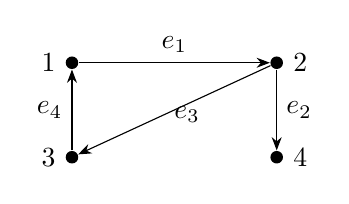
\begin{tikzpicture}[>=Stealth, baseline=(current bounding box.center)]
  \node[circle, fill=black, inner sep=1.6pt, label=left:$1$]  (v1) at (0,1.2) {};
  \node[circle, fill=black, inner sep=1.6pt, label=right:$2$] (v2) at (2.6,1.2) {};
  \node[circle, fill=black, inner sep=1.6pt, label=left:$3$]  (v3) at (0,0) {};
  \node[circle, fill=black, inner sep=1.6pt, label=right:$4$] (v4) at (2.6,0) {};

  % e1: 1 -> 2
  \draw[->] (v1) -- node[above] {$e_1$} (v2);

  % e2: 2 -> 4
  \draw[->] (v2) -- node[right] {$e_2$} (v4);

  % e3: 2 -> 3  (diagonal)
  \draw[->] (v2) -- node[pos=0.55, right] {$e_3$} (v3);

  % e4: 3 -> 1
  \draw[->] (v3) -- node[left] {$e_4$} (v1);
\end{tikzpicture}
\]
Show that there are more than one optimal strategies for Player~I in the corresponding
incidence matrix game.
\end{exercise}
\begin{proof}
\end{proof}
\end{document}